\section{Versuchsaufbau und Durchf"uhrung} % (fold)
\label{sec:durchf_uhrung}
	Es werden in diesem Versuch die W"armekapazit"aten $c_\mathrm{p}$ verschiedener Metalle bei konstantem Druck gemessen.
	Weil die Messung der W"armekapazit"at $c_\mathrm{V}$ bei konstantem Volumen schwierig ist, kann darauf mit dem Zusammenhang

	\begin{equation}
		c_\mathrm{p} - c_\mathrm{V} = 9 \alpha^2 \kappa V_0 T \,,
	\end{equation}

	geschlossen werden.
	Dabei bezeichnet $\alpha$ den linearen Ausdehnungskoeffizienten, $\kappa = V \partial_V \rho$ das Kompressionsmodul und $V_0$ das Molvolumen.

	\subsection{Mischungskaloriemeter}
	\label{subsec:kaloriemeter}
		Die Messung erfolgt mit Hilfe eines Mischungskaloriemeters.
		Eine r"ohrenf"ormige Probe wird dabei im Wasserbad erhitzt.
		Die heisse Probe der Masse $m_\mathrm{k}$ wird dann in ein mit einer Wassermenge $m_\mathrm{W}$ bef"ulltes Dewargef"a"s getaucht.
		Nach etwa einer Minute unter leichtem R"uhren, sind die Temperatur endes Wassers $T_\mathrm{W}$ und der Probe $T_\mathrm{k}$ angeglichen und es stellt sich die Mischtemperatur $T_\mathrm{m}$ ein.
		Zus"atzlich hat das Gef"a"s eine bestimmte W"armemenge $Q_\mathrm{g}$ aufgenommen, die ber"ucksichtigt werden muss.
		Unter der N"aherung, dass die Messapparatur ein geschlossenes System darstellt -- die Umgebungsluft also keine Energie aufnimmt -- gilt f"ur die spezifische W"armekapazit"at $c_\mathrm{k}$ der Probe:

		\begin{equation}
			c_\mathrm{k} = \frac{\left(c_\mathrm{w}m_\mathrm{w} + c_\mathrm{g}m_\mathrm{g}\right)\left(T_\mathrm{m} - T_\mathrm{w} \right)}{m_\mathrm{k} \left(T_\mathrm{k} - T_\mathrm{m} \right)} \,. \label{ck}
		\end{equation}

		Die W"armekapazit"at $c_\mathrm{g}m_\mathrm{g}$ des Kaloriemeters wird dabei bestimmt, indem zwei gleiche Wassermengen $m_\mathrm{x}$ und $m_\mathrm{y}$ unterschiedlicher Temperatur $T_\mathrm{x} < T_\mathrm{y}$ im Gef"a"s gemischt werden.
		Das k"altere Wasser der Temperatur $T_\mathrm{x}$ befindet sich dabei schon im Kaloriemeter.
		Nachdem sich nach der Mischung eine Konstante Temperatur $T_\mathrm{z}$ eingestellt hat, l"asst sich die W"armekapazit"at des Kaloriemeters durch

		\begin{equation}
			c_\mathrm{g}m_\mathrm{g} = \frac{c_\mathrm{w}m_\mathrm{y}\left( T_\mathrm{y} - T_\mathrm{z}\right) - c_\mathrm{w}m_\mathrm{x} \left( T_\mathrm{z} - T_\mathrm{x} \right) }{T_\mathrm{z} - T_\mathrm{x}} \label{cg}
		\end{equation}

		bestimmen. Dabei ist die spezifische W"armekapazit"at von Wasser bekannt mit $c_\mathrm{w} = \SI{4.18}{\joule \per \gram \per \kelvin}$ \cite{anleitung} bei etwa $T = \SI{40}{\celsius}$.

	\subsection{Temperaturmessung mit Hilfe eines Thermoelementes}
	\label{subsec:thermoelement}
		\begin{wrapfigure}{r}{7cm}
			\centering
			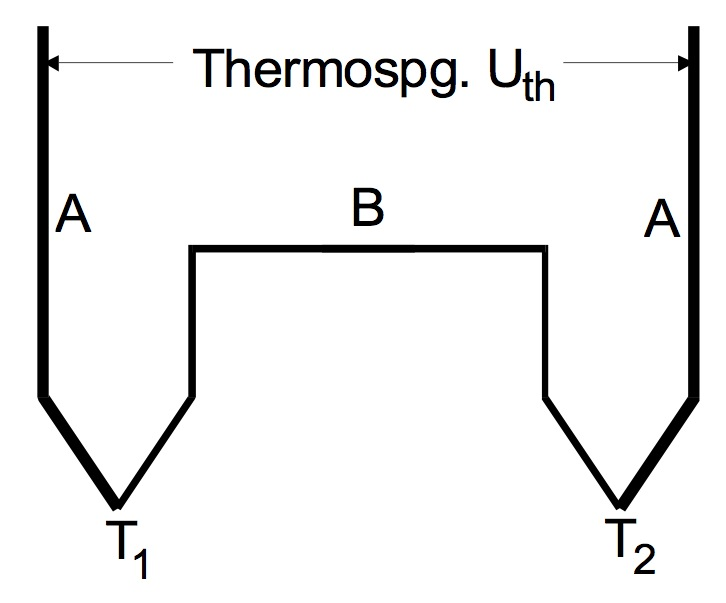
\includegraphics[width = 7cm]{img/thermoelement.jpg}
			\caption{Schematische Darstellung eines Thermoelements \cite{anleitung}.}
			\label{fig:thermoelement}
		\end{wrapfigure}

		Zur Temperaturmessung wird bei diesem Versuch ein Thermoelement genutzt.

		Zwei Metalle A und B mit verschiedener Elektronenaustrittsarbeit werden an zwei Stellen in Kontakt gebracht.
		Dort wandern die Ladungstr"ager vom Metall der geringeren Austrittsarbeit in das jeweils andere, bis sich ein Kontaktpotential einstellt, das den Elektronenfluss kompensiert.
		Eine Kontaktstelle wird ein Eiswasser getaucht und hat damit stets die Temperatur $T_1 = \SI{0}{\celsius}$, w"ahrend die andere Kontaktstelle zur Messung in das Kaloriemeter, bzw. das W"armebad getauch wird.

		Die Temperatur l"asst sich dann aus der anliegenden Spannung $U_\mathrm{th}$ errechnen, wobei sich empirisch der folgende Zusammenhang ergibt:

		\begin{equation}
			T = \SI{25.157}{} U_\mathrm{th} - \SI{.19}{} U_\mathrm{th}^2 \,. \label{T}
		\end{equation}

		Dabei ist zu beachten, dann die Temperatur $T$ nur im Bereich von $\SI{0}{\celsius}$ bis $\SI{100}{\celsius}$ gemessen werden k"onnen.

		\clearpage